\section{\label{sec:level1}Theoretical Background}
The most stable frequency reference is atomic oscillators due to the unperturbed clock transition being indistinguishable between atoms. Atomic clocks most commonly employ alkali atoms due to their well studied single valence electronic structure, high vapor pressure at room temperature and the D-lines$^[$\citep{Steck1998CesiumData}$^]$ being accessible using diode lasers. 
\begin{figure}[t]
\centering
\includegraphics[width=0.45\textwidth,keepaspectratio]{expsetup}
\caption{\label{fig:expsetup}CSAC CPT schematic with the LO, physics package and control electronics.}
\end{figure}
The hyperfine states of the atoms are further split by the Zeeman effect into the Zeeman sub-levels, $m_{f}$ in the presence of a magnetic field. The clock states are chosen as the hyperfine ground states, F=3 and F=4 when $m_{f}$=0, ($\ket{F=3,m_{f}=0}$-$\ket{F=4,m_{f}=0}$). This is due to the transition between $m_{f}$=0 sub-levels being insensitive to magnetic fields to the first order. The transition frequency is calculated as the difference in energy between the clock states divided by Planck's constant $^[$\citep{Knappe2007MEMSClocks}$^,$\citep{LombardiM.A.andHeavnerT.PandJefferts2007NISTSI}$^,$\citep{Sherlock2009HowSpectroscopy}$^]$.

%cesium over rubidium for the alkali metal in the physics
%package permits the resonance cell to operate optimally at
%70-80°C and leads naturally to integrating the VCSEL with
%the resonance cell. firmware algorithms  


The local oscillator (LO), the physics package and the control electronics are the main components of a CSAC $^[$\citep{Knappe2007MEMSClocks}$^]$. The physics package contains the spectroscopic setup, for the case shown in Fig. (\ref{fig:expsetup}) the technique used is coherent population trapping (CPT). CPT transmission peak occurs at the frequency of the transition between the clock states and is used as the reference frequency for the LO. A small internal magnetic field $B$ is applied to the atoms in the vapor cell to deflect the $m_{f}\neq$0 sub-levels from the clock states. Magnetic shielding prevents external magnetic fields reaching the vapour cell. Miniaturisation of the physical package and the vapor cell is completed using the micro-electro-mechanical system (MEMS) technology $^[$\citep{Wang2014ReviewTrapping}$^]$. Buffer gas is added to the cell containing the alkali droplet to decrease the broadening due to collisions with the cell walls. However, pressure broadening shifts the hyperfine ground state but this can be corrected by adding a second buffer gas which produces an opposite pressure broadening ground state shift $^[$\citep{Lutwak2002TheInterrogation}$^]$. The vertical-cavity surface-emitting laser (VCSEL) is used due to the high modulation bandwidth $^[$\citep{Knappe2007MEMSClocks}$^]$. The control electronics are used to apply corrections to the laser frequency, LO frequency, laser temperature and vapour cell temperature. The laser frequency and the cell temperature are controlled using servo loops. 


\subsection{Coherent population trapping (CPT)}


\begin{figure}[t]
\centering
\includegraphics[height=0.23\textwidth,keepaspectratio]{lambdatransition}
\caption{\label{fig:lambdatransition}The three-level $\Lambda$ configuration of separate electric fields driving the $\ket{1}-\ket{3}$ and $\ket{2}-\ket{3}$ transitions.}
\end{figure}

Commercially available CSACs currently exploit CPT phenomenon $^[$\citep{articleb}$^]$. The $\Lambda$ configuration as shown in Fig. (\ref{fig:lambdatransition}) approximates the alkali atoms as a three-level system with separate electric fields driving $\ket{1}-\ket{3}$ and $\ket{2}-\ket{3}$ transitions. Parity of the ground states forbids $\ket{1}-\ket{2}$ transitions $^[$\citep{Khan2017CoherentEIT}$^]$. CPT occurs in a $\Lambda$ system when the relative detuning $\Delta=\delta_{31}-\delta_{32}=0$ of the electric fields enables pumping into a non-coupled coherent state $\ket{NC}$ $^[$\citep{Phillips:05}$^]$. 

The atom-light interaction for a two-level system where the interaction Hamiltonian in the dipole approximation is $\hat{H}_{I}=-\hat{\vec{d}}\cdot\hat{\vec{E}}$ where $\hat{\vec{d}}$ is the electric dipole moment and the electric field operator is $\hat{\vec{E}}=\hat{\vec{\epsilon}}E_{0}cos(\omega t)$. The Rabi frequency is derived as $\Omega=\frac{E_{0}}{\hbar}\bra{e}\hat{\vec{d}}\cdot\hat{\vec{\epsilon}}\ket{g}$. By extending the derivation to a $\Lambda$ system the approximate non-coupled dark state can be calculated. The Hamiltonian $H=H_{0}+H_{I1}+H_{I2}$ is derived as 
\begin{equation}
\label{eq:interactionham0}
\hat{H}_{0}=\sum_{i}\hbar\omega_{i}\ket{i}\bra{i},
\end{equation}
\begin{equation}
\label{eq:interactionham1}
\hat{H}_{I1}=\frac{\hbar\Omega_{31}}{2}(e^{i\omega_{31}t}\ket{3}\bra{1}+e^{-i\omega_{31}t}\ket{1}\bra{3}),
\end{equation}
\begin{equation}
\label{eq:interactionham2}
\hat{H}_{I2}=\frac{\hbar\Omega_{32}}{2}(e^{i\omega_{32}t}\ket{3}\bra{2}+e^{-i\omega_{32}t}\ket{2}\bra{3}),
\end{equation}


where $\hat{H}_{0}$ is the internal energy of the atoms $^[$\citep{Purves2006AbsorptionInterferometery}$^]$ . The eigenstates of $\hat{H}$ when $\omega_{31}-\omega_{32}=\omega_{hfs}$ are derived as $^[$\citep{Purves2006AbsorptionInterferometery}$^]$: THIS

\begin{equation}
\label{eq:CPTstatesC1}
\ket{C_{1}}=\frac{1}{\sqrt[]{2}}(\frac{\Omega_{31}}{\sqrt[]{\Omega_{31}^{2}+\Omega_{32}^{2}}}\ket{1}+\frac{\Omega_{32}}{\sqrt[]{\Omega_{31}^{2}+\Omega_{32}^{2}}}\ket{2}-\ket{3}),
\end{equation}
\begin{equation}
\label{eq:CPTstatesC2}
\ket{C_{1}}=\frac{1}{\sqrt[]{2}}(\frac{\Omega_{31}}{\sqrt[]{\Omega_{31}^{2}+\Omega_{32}^{2}}}\ket{1}+\frac{\Omega_{32}}{\sqrt[]{\Omega_{31}^{2}+\Omega_{32}^{2}}}\ket{2}+\ket{3}),
\end{equation}
\begin{equation}
\label{eq:CPTstatesNC}
\ket{NC}=\frac{\Omega_{32}\ket{1}-\Omega_{31}\ket}{\sqrt[]{\Omega_{31}^{2}+\Omega_{32}^{2}}}.
\end{equation}

Since $\ket{NC}$ is a superposition of the ground states, atoms pumped into this dark state become trapped. Population builds up in the dark state and eventually the atoms do not interact with the electric fields. The  transmission peak is observed at $\omega_{hfs}$. This simplified derivation does not fully describe the system, it is important to note that phase coherence between the electric fields is a requirement for CPT $^[$\citep{Khan2017CoherentEIT}$^]$. The evolution of the three-level system is derived using the Lindblad Master equation in Ref. [\citen{5423}] and Ref. [\citen{Fleischhauer2005ElectromagneticallyMedia}]. In ref. [\citen{Borges2017InfluenceTrapping}] the first order optical susceptibility $\chi^{(1)}$ is calculated, where $\chi^{(1)}$ applies for CPT and the typical regime of electromagnetically induced transparency (EIT) ($\Omega_{31}\gg \Omega_{32}$). The system absorption and dispersion is given by \textit{Im}$(\chi^{(1)})$ and \textit{Re}$(\chi^{(1)})$, respectively. 


Fig. (\ref{fig:CPTplot}) shows the absorption and dispersion plotted as a function of the relative detuning $\Delta=\omega_{31}-\omega_{32}-\omega_{hfs}$ where the sharp transmission peak at zero detuning enables locking of the LO to ground state resonance. This is experimentally achieved using a current-modulated diode laser which has an optical carrier frequency and a modulated frequency of $\omega_{hfs}/2$ to produce the first order sidebands separated by $\omega_{hfs}$. The laser frequency is tuned such that the first-order sidebands are resonant with the $\ket{1}-\ket{3}$ and $\ket{2}-\ket{3}$ transition $^[$\citep{Lutwak2002TheInterrogation}$^]$. 

\begin{figure}[t]
\centering
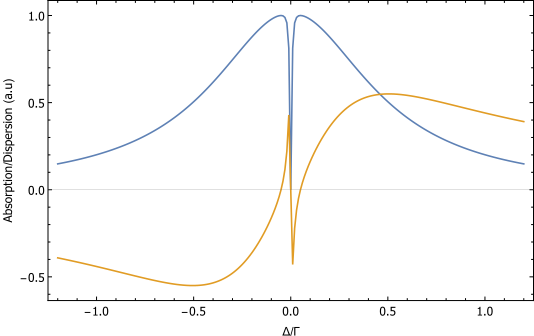
\includegraphics[height=0.27\textwidth,keepaspectratio]{CPTplot}
\caption{\label{fig:CPTplot}Theoretical absorption (blue) and dispersion (yellow/brown) as a function of $\Delta/\Gamma$ in the CPT regime ($\Omega_{31}\approx\Omega_{32}$) where $0.5\Gamma=\Gamma_{31}=\Gamma_{32}$.}
\end{figure}


\subsection{Frequency Stability}
Accuracy and stability are characteristics of an oscillator. Accuracy describes the offset from the ideal value, whilst stability defines the ability to produce the same value over a certain period of time $^[$\citep{Lombardi2001AnCalibrations}$^]$. The performance of CSACs relies upon the frequency stability over a certain integration time, the power consumption and the size of the device. The Allan deviation $\sigma_{y}$ provide a measure of the fractional frequency stability. In Ref. [\citen{Knappe2007MEMSClocks}] white frequency noise approximately describes the frequency stability when the averaging time $\tau$<100 s, such that:

\begin{equation}
\label{eq:AllanDev}
\sigma_{y}(\tau)=\frac{X}{Q(S/N)}\sqrt[]{\tau}.
\end{equation}

It is clear from Eq. (\ref{eq:AllanDev}) that frequency stability is dependent on the Lorentzian CPT transmission linewidth $\gamma$ and the amplitude.   
The quality factor $Q=\omega_{c} /\gamma$, the signal to noise ratio is $S/N$ and $X$ is the method of interrogation parameter. In addition, frequency stability depends on, for the case of $\tau\approx100 s$ and $\tau>100$ s the flicker noise floor ($\sigma_{y}\propto const$) and the frequency drift ($\sigma_{y}\propto\tau$), respectively.  

\begin{figure}[t]
\centering
\includegraphics[height=0.37\textwidth,keepaspectratio]{frequencystability}
\caption{\label{fig:frequencystability} $\sigma_{y}$ of the locked oscillator (red) and for unlocked free-running oscillator (green). The atomic stability (black dashes) is modelled by the white noise (grey dots), flicker noise floor (blue dashes) and frequency drift (orange dot dashes) \citep{Knappe2007MEMSClocks}.}
\end{figure}



